\documentclass[xcolor=x11names, aspectratio=169,usenames,dvipsnames]{beamer}
\usepackage[british]{babel}
\usepackage{amsmath}
\usepackage{amssymb}
\usepackage{amsfonts}
\usepackage{mathpazo}
\usepackage{enumerate}
\usepackage{array,booktabs}
\usepackage{tikz}
\usepackage{mathdots}
\usepackage{verbatim}
\usepackage{multirow}
\usepackage{tabularx}
\usetikzlibrary{matrix,backgrounds,patterns,arrows,decorations.markings,shapes,positioning}
\usepackage{caption}

\usetheme[titleformat title=regular,titleformat frame=regular,titleformat section=allcaps,numbering=fraction]{metropolis}

\author[F.\ Kußmaul \&\ T.\ Evans]{{\Large Felix Kußmaul}\hfill\raisebox{-.9em}{
\includegraphics[width=4cm]{img/uco.jpg}}\\[1.2em]{\Large Dr Tim Evans}\hfill\raisebox{-.7em}{
\includegraphics[width=4cm]{img/york.jpg}}}
\title[Mining Paper Catalogues]{\Large Mining Paper Catalogues}
\subtitle{\normalsize A Multilingual Solution to Reduce Verbose Fields to Consistent Terminology}
\institute[Cologne, York]{European Association of Archaeologists 2017}
\date[31 August 2017]{\ \\[.5em]31 August 2017}

\usepackage{pdfrender}

\newcommand{\red}[1]{\textcolor{red}{#1}}
\newcommand{\orange}[1]{\textcolor{orange}{#1}}
\newcommand{\green}[1]{\textcolor{markgreen}{#1}}
\newcommand{\textgreen}[1]{\textcolor{textgreen}{#1}}
\newcommand{\blue}[1]{\textcolor{textblue}{#1}}
\newcommand{\gray}[1]{\textcolor{gray}{#1}}

\newcolumntype{R}{>{\centering\raggedleft\arraybackslash}X}
\newcolumntype{L}{>{\centering\raggedright\arraybackslash}X}
\newcolumntype{C}{>{\centering\arraybackslash}X}

\usepackage[style=authortitle-comp,backend=biber]{biblatex}
\addbibresource{eaa.bib}
\renewcommand*{\bibfont}{\small}

\setbeamercovered{transparent}

\newcommand{\textsb}[1]{{\fontfamily{cmss}\fontseries{sbc}\fontshape{n}\selectfont #1}}

\setbeamertemplate{enumerate items}[square]

\setbeamertemplate{footline}
{
\hbox{%
  \begin{beamercolorbox}[wd=.26\paperwidth,ht=2.7ex,dp=1.2ex,center]{author in head/foot}%
    \usebeamerfont{author in head/foot}\insertshortauthor\ (\insertshortinstitute)
  \end{beamercolorbox}%
  \begin{beamercolorbox}[wd=.40\paperwidth,ht=2.7ex,dp=1.2ex,center]{author in head/foot}%
    \usebeamerfont{title in head/foot}\insertshorttitle:\ \textbf{\insertsection}
  \end{beamercolorbox}%
  \begin{beamercolorbox}[wd=.36\paperwidth,ht=2.7ex,dp=1.2ex,center]{author in head/foot}%
    \usebeamerfont{date in head/foot}\insertshortdate\hfill\insertframenumber/\inserttotalframenumber\strut
  \end{beamercolorbox}}
  \vskip0pt%
}

\tikzset{
  invisible/.style={opacity=0},
  visible on/.style={alt={#1{}{invisible}}},
  alt/.code args={<#1>#2#3}{%
    \alt<#1>{\pgfkeysalso{#2}}{\pgfkeysalso{#3}} % \pgfkeysalso doesn't change the path
  },
}

%\newcommand{\printSectionYes}{\AtBeginSection[]
%{
% \begin{frame}{Agenda}
% \tableofcontents[sectionstyle=show/shaded,
% 					subsectionstyle=show/shaded/hide]
% \end{frame}
%}}

\tikzset{onslide/.code args={<#1>#2}{%
  \only<#1>{\pgfkeysalso{#2}}%
}}

\setbeamertemplate{section in toc shaded}[default][50]

\setbeamertemplate{subsection in toc shaded}[default][50]

\makeatletter
\patchcmd{\beamer@sectionintoc}{\vskip1.5em}{\vskip0.5em}{}{}
\makeatother

\makeatletter
\newcommand\footnoteref[1]{\protected@xdef\@thefnmark{\ref{#1}}\@footnotemark}
\makeatother

\setbeamertemplate{bibliography item}{%
  \ifboolexpr{ test {\ifentrytype{book}} or test {\ifentrytype{mvbook}}
    or test {\ifentrytype{collection}} or test {\ifentrytype{mvcollection}}
    or test {\ifentrytype{reference}} or test {\ifentrytype{mvreference}} }
    {\setbeamertemplate{bibliography item}[book]}
    {\ifentrytype{online}
       {\setbeamertemplate{bibliography item}[online]}
       {\setbeamertemplate{bibliography item}[article]}}%
  \usebeamertemplate{bibliography item}}
  
\defbibenvironment{bibliography}
  {\list{}
     {\settowidth{\labelwidth}{\usebeamertemplate{bibliography item}}%
      \setlength{\leftmargin}{\labelwidth}%
      \setlength{\labelsep}{\biblabelsep}%
      \addtolength{\leftmargin}{\labelsep}%
      \setlength{\itemsep}{\bibitemsep}%
      \setlength{\parsep}{\bibparsep}}}
  {\endlist}
  {\item}
  
%%% DEFINE DOCUMENT SHAPE
% taken from manual
\makeatletter
\pgfdeclareshape{document}{
\inheritsavedanchors[from=rectangle] % this is nearly a rectangle
\inheritanchorborder[from=rectangle]
\inheritanchor[from=rectangle]{center}
\inheritanchor[from=rectangle]{north}
\inheritanchor[from=rectangle]{south}
\inheritanchor[from=rectangle]{west}
\inheritanchor[from=rectangle]{east}
% ... and possibly more
\backgroundpath{% this is new
% store lower right in xa/ya and upper right in xb/yb
\southwest \pgf@xa=\pgf@x \pgf@ya=\pgf@y
\northeast \pgf@xb=\pgf@x \pgf@yb=\pgf@y
% compute corner of ‘‘flipped page’’
\pgf@xc=\pgf@xb \advance\pgf@xc by-5pt % this should be a parameter
\pgf@yc=\pgf@yb \advance\pgf@yc by-5pt
% construct main path
\pgfpathmoveto{\pgfpoint{\pgf@xa}{\pgf@ya}}
\pgfpathlineto{\pgfpoint{\pgf@xa}{\pgf@yb}}
\pgfpathlineto{\pgfpoint{\pgf@xc}{\pgf@yb}}
\pgfpathlineto{\pgfpoint{\pgf@xb}{\pgf@yc}}
\pgfpathlineto{\pgfpoint{\pgf@xb}{\pgf@ya}}
\pgfpathclose
% add little corner
\pgfpathmoveto{\pgfpoint{\pgf@xc}{\pgf@yb}}
\pgfpathlineto{\pgfpoint{\pgf@xc}{\pgf@yc}}
\pgfpathlineto{\pgfpoint{\pgf@xb}{\pgf@yc}}
\pgfpathlineto{\pgfpoint{\pgf@xc}{\pgf@yc}}
}
}
\makeatother


%\setbeamertemplate{title page}{%
%\begin{tikzpicture}[remember picture,overlay]
%\fill[orange]
%  ([yshift=15pt]current page.west) rectangle (current page.south east);
%\node[anchor=east] 
%  at ([yshift=-50pt]current page.north east) (author)
%  {\parbox[t]{.6\paperwidth}{\raggedleft%
%    \usebeamerfont{author}\textcolor{orange}{%
%    \textpdfrender{
%    TextRenderingMode=FillStroke,
%    FillColor=orange,
%    LineWidth=.1ex,
%    }{\insertauthor}}}};
%\node[anchor=north east] 
%  at ([yshift=-70pt]current page.north east) (institute)
%  {\parbox[t]{.78\paperwidth}{\raggedleft%
%    \usebeamerfont{institute}\textcolor{gray}{\insertinstitute}}};
%\node[anchor=south west] 
%  at ([yshift=20pt]current page.west) (logo)
%  {\parbox[t]{.19\paperwidth}{\raggedleft%
%    \usebeamercolor[fg]{titlegraphic}\inserttitlegraphic}};
%\node[anchor=east]
%  at ([yshift=-10pt,xshift=-20pt]current page.east) (title)
%  {\parbox[t]{\textwidth}{\raggedleft%
% \usebeamerfont{author}\textcolor{white}{%
%    \textpdfrender{
%    TextRenderingMode=FillStroke,
%    FillColor=white,
%    LineWidth=.1ex,
%    }{\inserttitle}}}};
%\node[anchor=east]
%  at ([yshift=-60pt,xshift=-20pt]current page.east) (subtitle)
%  {\parbox[t]{.6\paperwidth}{\raggedleft\usebeamerfont{subtitle}\textcolor{black}{\insertsubtitle}}};
%\end{tikzpicture}
%}
\definecolor{morange}{HTML}{FF8200}
 
\begin{document}

\maketitle

\section{Motivation}

\begin{frame}{Data Source}
\begin{center}
\begin{figure}
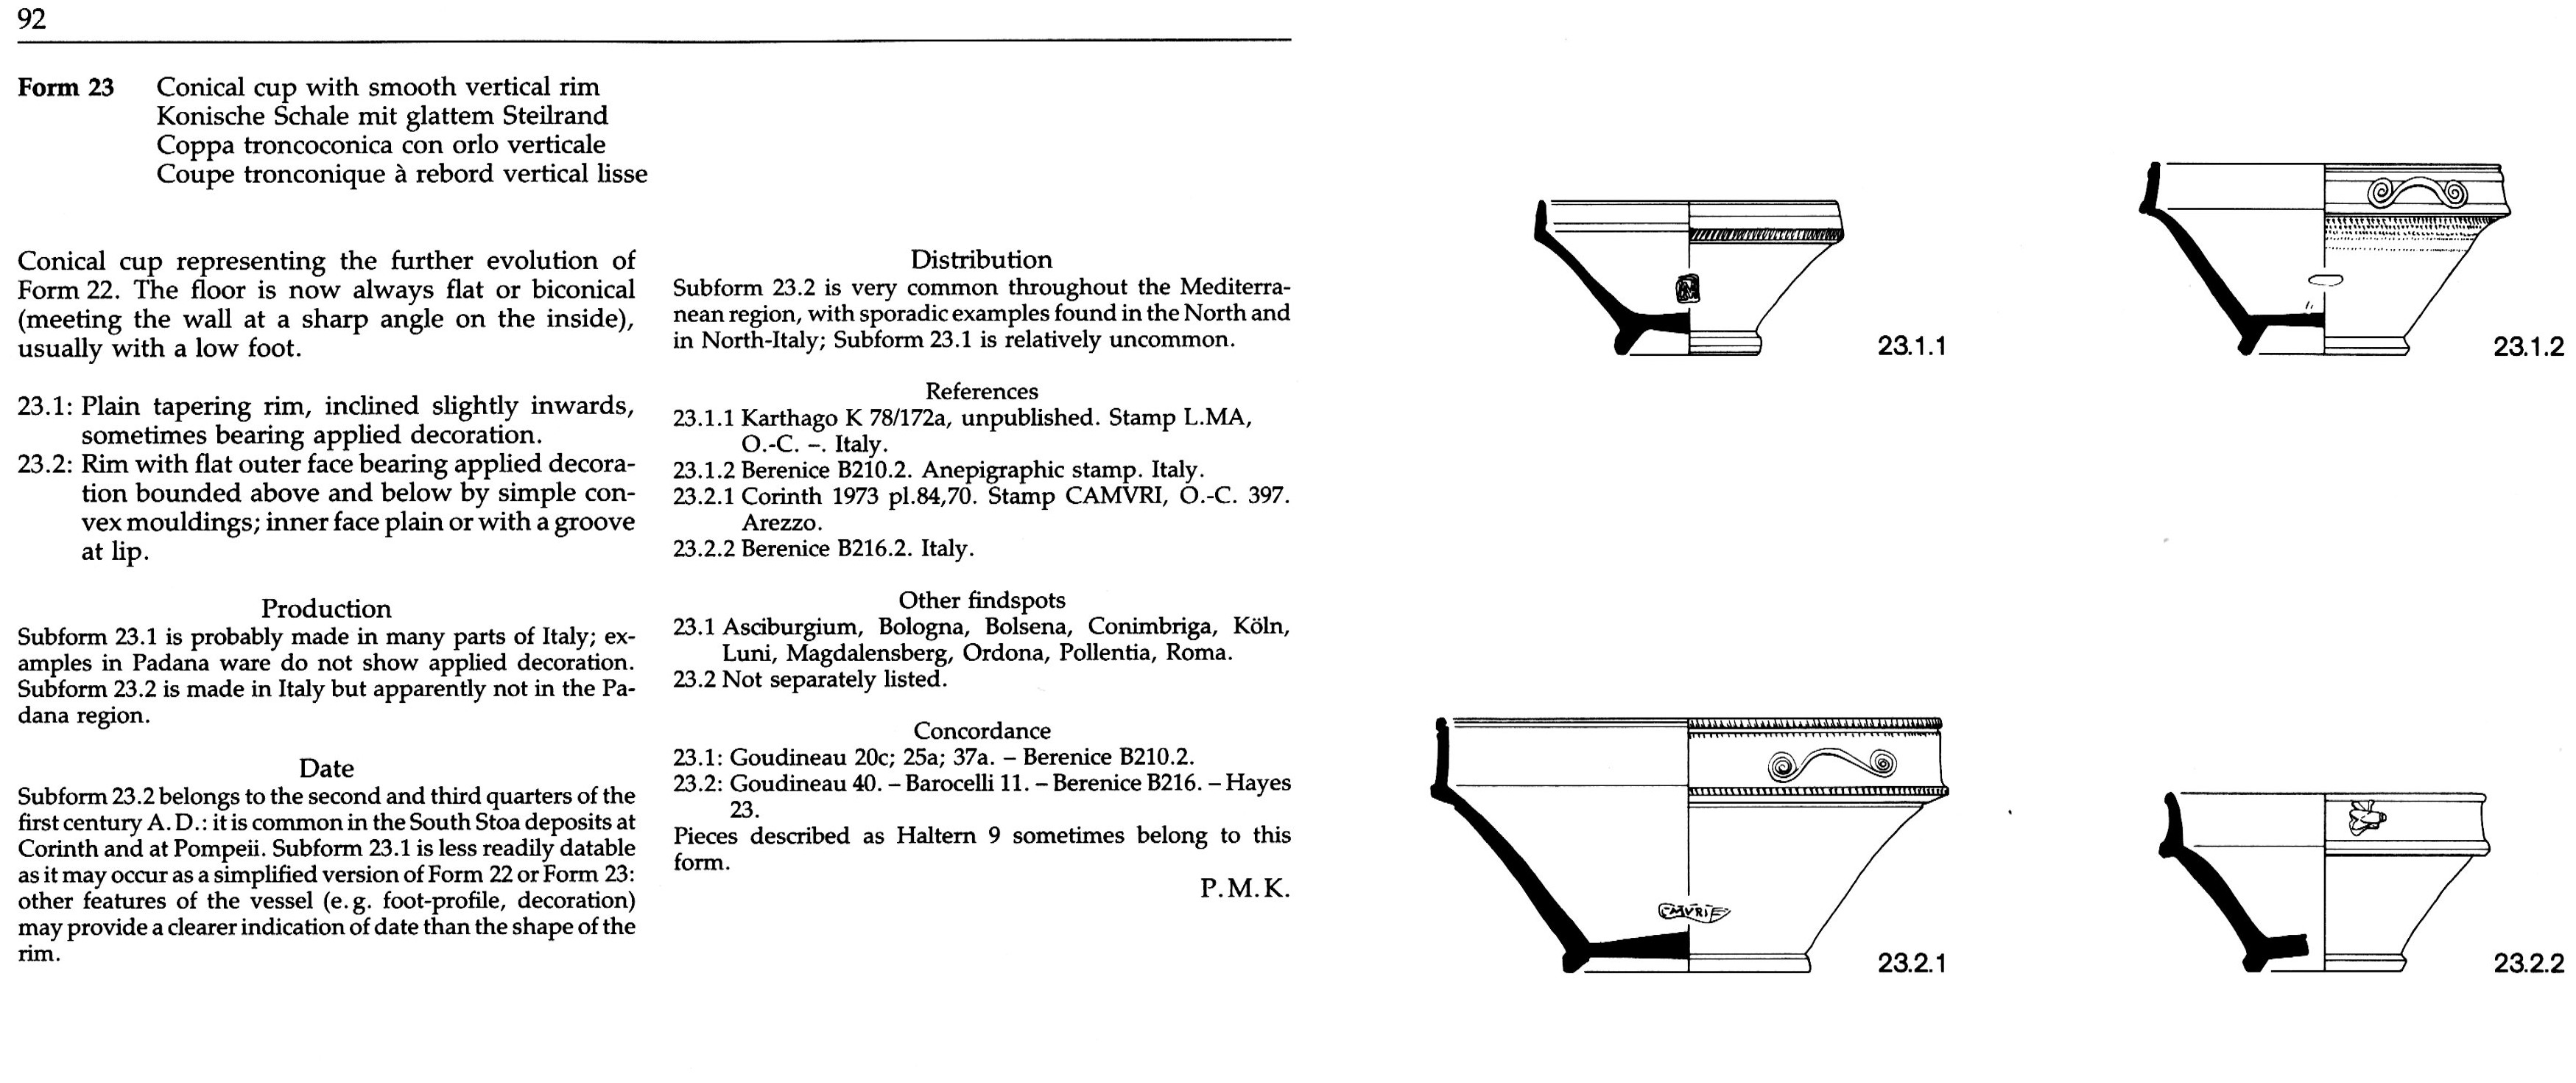
\includegraphics[width=.875\paperwidth]{img/consp.jpg}
\caption{Sample from \emph{Conspectus} catalogue.}
\end{figure}
\end{center}
\end{frame}

\begin{frame}[fragile]{}
\begin{minipage}[t]{0.45\textwidth}
What we \textbf{have}:\medskip

\begin{figure}
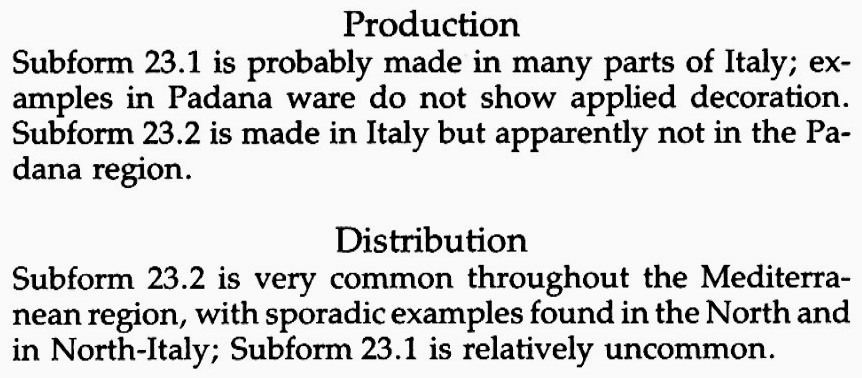
\includegraphics[width=1.0\textwidth]{img/consp_ex.jpg}
\end{figure}
\end{minipage}\hfill\pause
\begin{minipage}[t]{0.45\textwidth}
What we \textbf{want}:\medskip
{\scriptsize
\begin{verbatim}
{
   "form": "23.1",
   "origin": "Italy",
   "decoration": "none",
   "occurs": "uncommon"
},
{
   "form": "23.2",
   "origin": "Italy, not Padana",
   "occurs": "Mediterranean region;
              North-Italy"
}
\end{verbatim}
}
\end{minipage}\pause\medskip

\begin{minipage}[t]{0.45\textwidth}
\begin{center}
\alert{\textbf{UNSTRUCTURED DATA}}
\end{center}
\end{minipage}\hfill
\begin{minipage}[t]{0.45\textwidth}
\begin{center}
\alert{\textbf{STRUCTURED DATA}}
\end{center}
\end{minipage}

\end{frame}

\begin{frame}
\begin{tabbing}
\qquad\textbf{Problem:} \= Running texts contain a lot of \alert{irrelevant information}.\\[.5em]

\> Information scientists call them \textbf{redundant}.
\end{tabbing}
\end{frame}

{ % all template changes are local to this group.
	\setbeamercolor{background canvas}{bg=black}
    \setbeamertemplate{navigation symbols}{}
    \begin{frame}[plain]
        \begin{tikzpicture}[remember picture,overlay]
            \node[at=(current page.center)] {
                
\includegraphics[height=\paperheight]{img/death.jpg}
            };
        \end{tikzpicture}
     \end{frame}
}

\section{Text Mining: Theory}%\printSectionYes

\begin{frame}{Classification}
\textbf{Text Mining} is a \alert{general term} covering several different ideas, e.\,g.:\pause

\begin{itemize}[<+->]
\item Information retrieval
\item Cluster analysis
\item Statistical (lexical) analysis
\item \textbf{Information extraction}
\item\dots
\end{itemize}
\end{frame}

\begin{frame}{Information Extraction}
\textbf{Information extraction} (IE) is the task of automatically extracting structured information from unstructured [\dots] documents.\pause\bigskip

Information extraction is \textbf{\alert{really fucking hard}}.
\end{frame}

\begin{frame}{IE: Five Steps}
\begin{enumerate}
\item Tokenisation and Sentence splitting
\item Lemmatisation
\item Part-of-speech-tagging (POS)
\item Named entity recognition (NER)
\item Relation Extraction
\end{enumerate}
\end{frame}

\begin{frame}{POS-Tagging}
\begin{figure}
\tikzstyle{block} = [rectangle, draw, fill=blue!10, rounded corners, text centered, minimum width=1.5em,font=\footnotesize\ttfamily, node distance=2em]
\begin{tikzpicture}[node distance = .5em, font=\bfseries\large,baseline, text height=1.5ex,text depth=.25ex,highlight/.style={text=orange}]
\node (a) at (0,0) {The};
\node[right=of a,onslide={<2-> highlight}] (b) {quick};
\node[right=of b,onslide={<2-> highlight}] (c) {brown};
\node[right=of c,onslide={<2-> highlight}] (d) {fox};
\node[right=of d] (e) {jump};
\node[right=of e] (f) {over};
\node[right=of f] (g) {the};
\node[right=of g,onslide={<2-> highlight}] (h) {lazy};
\node[right=of h,onslide={<2-> highlight}] (i) {dog};
\node[right=of i] (j) {.};

\node[block,fill=Fuchsia!30,below of=a] {DT};
\node[block,fill=yellow!30,below of=b] {JJ};
\node[block,fill=yellow!30,below of=c] {JJ};
\node[block,fill=RoyalBlue!30,below of=d] {NN};
\node[block,fill=green!30,below of=e] {VBD};
\node[block,fill=orange!30,below of=f] {IN};
\node[block,fill=Fuchsia!30,below of=g] {DT};
\node[block,fill=yellow!30,below of=h] {JJ};
\node[block,fill=RoyalBlue!30,below of=i] {NN};
\node[block,fill=gray!30,below of=j] {.};

\node at (0,-1.5) {};
\node[above of=e,gray,node distance=1.3em,font=\mdseries] {\footnotesize jumps}; 
\end{tikzpicture}
\caption{POS-tagging examples after lemmatisation.}
\end{figure}
\end{frame}

\begin{frame}{POS-Tagging}
\begin{figure}
\tikzstyle{block} = [rectangle, draw, fill=blue!10, rounded corners, text centered, minimum width=1.5em,font=\footnotesize\ttfamily, node distance=2em]
\begin{tikzpicture}[node distance = .2em, font=\bfseries,baseline, text height=1.5ex,text depth=.25ex,highlight/.style={text=orange}]
\node[onslide={<2> highlight}] (a) at (0,0) {Form};
\node[right=of a,onslide={<2> highlight}] (b) {20};
\node[right=of b] (c) {occur};
\node[right=of c] (f) {from};
\node[right=of f] (g) {the};
\node[right=of g,onslide={<2> highlight}] (h) {Augustan};
\node[right=of h] (i) {until};
\node[right=of i] (j) {the};
\node[right=of j,onslide={<2> highlight}] (k) {late};
\node[right=of k,onslide={<2> highlight}] (l) {Tiberian};
\node[right=of l,onslide={<2> highlight}] (m) {period};
\node[right=of m] (n) {.};

\node[block,fill=RoyalBlue!30,below of=a] {NN};
\node[block,fill=Fuchsia!30,below of=b] {CD};
\node[block,fill=green!30,below of=c] {VBZ};
\node[block,fill=orange!30,below of=f] {IN};
\node[block,fill=Fuchsia!30,below of=g] {DT};
\node[block,fill=RoyalBlue!30,below of=h] {NNP};
\node[block,fill=orange!30,below of=i] {IN};
\node[block,fill=Fuchsia!30,below of=j] {DT};
\node[block,fill=yellow!30,below of=k] {JJ};
\node[block,fill=yellow!30,below of=l] {JJ};
\node[block,fill=RoyalBlue!30,below of=m] {NN};
\node[block,fill=gray!30,below of=n] {.};

\node at (0,-1.5) {};
\node[above of=c,gray,node distance=1.2em,font=\mdseries] {\footnotesize occurs};
\end{tikzpicture}
\caption{POS-tagging examples after lemmatisation.}
\end{figure}
\end{frame}

\begin{frame}{Relation Extraction}
\begin{center}
\begin{tabularx}{\textwidth}{CCC}
\toprule
\textbf{Subject}&\textbf{Relation}&\textbf{Object}\\\midrule
quick brown fox&jump over&lazy dog\\
Form 20&occur&Augustan\\
Form 20&occur&late Tiberian period\\
\bottomrule
\end{tabularx}
\end{center}
\end{frame}

\section{Text Mining: Practical}

\begin{frame}[fragile]{Stanford CoreNLP: Output}
\begin{quote}
Subform 20.1 is never common, but has a long history from the Augustan period until the late Tiberian or early Claudian period.
\end{quote}
results in
\begin{verbatim}
have history until: Subform 20.1, tiberian
have history until: Subform 20.1, late tiberian
have history until: Subform, tiberian
have history until: Subform, late tiberian
\end{verbatim}
\end{frame}

\section{Multilingualism}

\maketitle

\end{document}
